\documentclass[tikz]{standalone}
\usetikzlibrary{angles,arrows,backgrounds,quotes}
\tikzstyle{background grid}=[draw, step=0.2cm, gray, very thin]

% Colors
\colorlet{veccol}{black!30}
% Vector styles
\tikzstyle{vec}=[-stealth,line cap=round,veccol]
\tikzstyle{vecdash}=[dash pattern=on 2pt off 1pt,very thin,
veccol,line cap=round]

\begin{document}

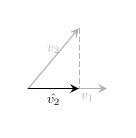
\begin{tikzpicture}[every node/.style={scale=0.5}]
  % [show background grid]
  \coordinate (O) at (0,0);
  \coordinate (A) at (1,0);
  \coordinate (B) at (50:1);
  \coordinate (C) at (B |- O);
  % Vectors
  \draw[vecdash] (B) -- (C);
  \draw[vec] (O) -- node [below,near end] {\(v_{1}\)} (A);
  \draw[vec] (O) -- node [above] {\(v_{2}\)} (B);
  \draw[vec,black] (O) -- node [below] {\(\hat{v_{2}}\)} (C);
\end{tikzpicture}

\end{document}


%%% Local Variables:
%%% mode: latex
%%% TeX-master: t
%%% End:
